% vim: foldmethod=marker foldlevel=0

% -----------------------------------------------------------------------------
% information
% -----------------------------------------------------------------------------

\def \docAuthor {\question{Name:}\answer{Answer Key}}
\def \docClass  {CPSC 120}
\def \docSchool {~}
\def \docTerm   {Spring 2014}
\def \docTitle  {Worksheets}


% -----------------------------------------------------------------------------
% document setup
% -----------------------------------------------------------------------------
% {{{

\documentclass[12pt,letterpaper]{article}

\usepackage[includehead,
            includefoot,
            margin=1in,
            top=.25in,
            headheight=.75in,
            headsep=.25in,
            footskip=.25in,
           ]{geometry}

\usepackage[fleqn]{amsmath}
\usepackage{amssymb}
\usepackage{array}
\usepackage{enumitem}
\usepackage{fancybox}
\usepackage{fancyhdr}
\usepackage{l3regex}
\usepackage{mathtools}
\usepackage{minted}
\usepackage{multicol}
\usepackage{tikz}
\usepackage[normalem]{ulem}
\usepackage{url}
\usepackage{xcolor}


% text ------------------------------------------------------------------------

\binoppenalty = 10000  % never break next to a binary operator
\relpenalty   = 10000  % never break next to a relation operator

\setlength{\parindent}{0em}
\setlength{\parskip}{1ex}

\setlist[itemize]{nosep,itemsep=.5ex,parsep=.5ex}

% math ------------------------------------------------------------------------

\setlength{\mathindent}{1cm}

% - "\begin{document}" resets these values, so they have to be treated
%   specially
\AtBeginDocument{
  \setlength{\abovedisplayskip}{1.5ex plus .5ex minus .5ex}
  \setlength{\belowdisplayskip}{1.5ex plus .5ex minus .5ex}
}

% source code -----------------------------------------------------------------

\usemintedstyle{solarizedlight}

% \fvset{samepage=true,frame=single,rulecolor=\color{.!30},framesep=2mm}
\fvset{samepage=true}

% header and footer -----------------------------------------------------------

\pagestyle{fancy}

\lhead{{\color{.}\docClass}}
\rhead{{\color{.}\docTitle}}
\lfoot{{\color{.}\docSection}}
\cfoot{{\color{.}\thepage}}
\rfoot{{\color{.}\docSubsection}}
\renewcommand{\headrule}{{\answer{\color{red}}\question{\color{.}}
                          \hrule height 0.4pt}}
\renewcommand{\footrule}{{\answer{\color{red}}\question{\color{.}}
                          \hrule height 0.4pt}}

\fancypagestyle{firstpage}{
  \fancyhead[L]{{\answer{\color{red}}\question{\color{.}}\docAuthor}
                {\color{.}\\\docClass}}
  \fancyhead[C]{{\color{.}\docSchool\\}}
  \fancyhead[R]{{\color{.}\docTerm\\\docTitle}}
  \fancyfoot[R]{}
}


% -----------------------------------------------------------------------------
% macros
% -----------------------------------------------------------------------------

% abbreviations ---------------------------------------------------------------

\def \<{\langle}
\def \>{\rangle}

\def \ε{\varepisilon}
\def \θ{\vartheta}
\def \κ{\varkappa}
\def \π{\varpi}
\def \ρ{\varrho}
\def \σ{\varsigma}
\def \φ{\varphi}

\def \Γ{\varGamma}
\def \Δ{\varDelta}
\def \Θ{\varTheta}
\def \Λ{\varLambda}
\def \Ξ{\varXi}
\def \Π{\varPi}
\def \Σ{\varSigma}
\def \Υ{\varUpsilon}
\def \Φ{\varPhi}
\def \Ψ{\varPsi}
\def \Ω{\varOmega}

% special characters ----------------------------------------------------------

\catcode `α = \active \let α \alpha
\catcode `β = \active \let β \beta
\catcode `γ = \active \let γ \gamma
\catcode `δ = \active \let δ \delta
\catcode `ε = \active \let ε \epsilon
\catcode `ζ = \active \let ζ \zeta
\catcode `η = \active \let η \eta
\catcode `θ = \active \let θ \theta
\catcode `ι = \active \let ι \iota
\catcode `κ = \active \let κ \kappa
\catcode `λ = \active \let λ \lambda
\catcode `μ = \active \let μ \mu
\catcode `ν = \active \let ν \nu
\catcode `ξ = \active \let ξ \xi
\catcode `ο = \active \let ο o
\catcode `π = \active \let π \pi
\catcode `ρ = \active \let ρ \rho
\catcode `σ = \active \let σ \sigma
\catcode `τ = \active \let τ \tau
\catcode `υ = \active \let υ \upsilon
\catcode `φ = \active \let φ \phi
\catcode `χ = \active \let χ \chi
\catcode `ψ = \active \let ψ \psi
\catcode `ω = \active \let ω \omega

\catcode `Α = \active \let Α A
\catcode `Β = \active \let Β B
\catcode `Γ = \active \let Γ \Gamma
\catcode `Δ = \active \let Δ \Delta
\catcode `Ε = \active \let Ε E
\catcode `Ζ = \active \let Ζ Z
\catcode `Η = \active \let Η H
\catcode `Θ = \active \let Θ \Theta
\catcode `Ι = \active \let Ι I
\catcode `Κ = \active \let Κ K
\catcode `Λ = \active \let Λ \Lambda
\catcode `Μ = \active \let Μ M
\catcode `Ν = \active \let Ν N
\catcode `Ξ = \active \let Ξ \Xi
\catcode `Ο = \active \let Ο O
\catcode `Π = \active \let Π \Pi
\catcode `Ρ = \active \let Ρ P
\catcode `Σ = \active \let Σ \Sigma
\catcode `Τ = \active \let Τ T
\catcode `Υ = \active \let Υ \Upsilon
\catcode `Φ = \active \let Φ \Phi
\catcode `Χ = \active \let Χ X
\catcode `Ψ = \active \let Ψ \Psi
\catcode `Ω = \active \let Ω \Omega

% }}}
% other -----------------------------------------------------------------------
% {{{

% - sometimes a "\par", especially at the end of a block, is necessary to
%   prevent an extra (empty) paragraph from appearing in the output
% - `\color{.!50}` means 50 percent of the current color

\newlength{\currentparskip}

\def \docSection {}
\def \docSubsection {}

\def \mysection #1{\section{#1} \gdef \docSection {#1}}
\def \mysubsection #1{\subsection*{#1} \gdef \docSubsection {#1}}

     \def \note     #1{{\color{.!50}#1\par}}
\long\def \longnote #1{{\color{.!50}#1\par}}

\def \ssQuestions {\mysubsection{Short Answer}}
\def \ssScope     {\mysubsection{Circle the Variables' Scopes}}
\def \ssMemory    {\mysubsection{Fill in the Memory}}
\def \ssFix       {\mysubsection{Fix the Broken Code}}
\def \ssTrace     {\mysubsection{Trace the Working Code}}

\long\def \textQuestion #1#2{%
  \setlength{\currentparskip}{\parskip}
  \begin{minipage}[t][3.5in][t]{\textwidth}
    \setlength{\parskip}{\currentparskip}
    \subsubsection*{Question}
    \vspace{-1ex}
    #1
    \vspace{-2ex}
    \subsubsection*{Answer}
    \vspace{-1ex}
    \answer{#2}
  \end{minipage}
}

\def \codeScope #1{%
  \vspace{1ex}
  \inputminted[fontsize=\large]{c++}{./code/#1.cpp}
  \newpage
}

\def \codeMemory #1{%
  \vspace{2ex}
  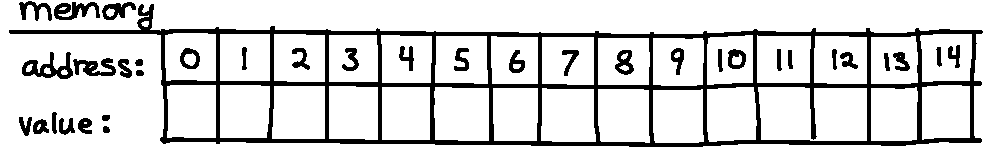
\includegraphics{./images/memory-0}
  \vspace{-2ex}
  \inputminted[fontsize=\large]{c++}{./code/#1.cpp}
  \newpage
}

\def \codeFix #1{%
  \question{
    \inputminted{c++}{./code/#1.cpp}
  } \answer{

    \inputminted[frame=single,rulecolor=\color{.!30},framesep=2mm]
                {c++}{./code/#1.answer.cpp}
    \vspace{-6ex}
    \inputminted[frame=single,rulecolor=\color{.!30},framesep=2mm]
                {diff}{./code/#1.answer.cpp.diff}
    \vspace{-6ex}
    \inputminted[frame=single,rulecolor=\color{.!30},framesep=2mm]
                {text}{./code/#1.answer.cpp.output}
  }
  \newpage
}

\def \codeTrace #1{%
  \inputminted{c++}{./code/#1.cpp}
  \question{
  } \answer{
    \vspace{-4ex}
    \inputminted[frame=single,rulecolor=\color{.!30},framesep=2mm]
                {text}{./code/#1.cpp.output}
  }
  \newpage
}


% }}}
% -----------------------------------------------------------------------------
% document
% -----------------------------------------------------------------------------

\begin{document}
\thispagestyle{firstpage}

\section*{Instructions}\gdef\docSection{Instructions}
For a each topic (if applicable) there are 5 sections:

\ssQuestions
Answer each question as well as you can.

\ssScope
Circle the scope of the given variables -- i.e., circle the part of the code in
which each variable ``exists''.  A good test, if you're not sure, is: if you
inserted a statement to \verb!cout! the variable at a given point in the code,
would any errors be produced?

\ssMemory
Fill in (or draw) a picture representing the computer memory, showing how the
variables might be allocated, and whether they have an assigned value, or are
uninitialized (use \verb!?! for ``uninitialized'').

\ssFix
Modify the code in the cleanest (and shortest) way possible, so that it will
compile and run without errors or warnings.

\ssTrace
Trace through the execution of the code, keeping track of the value of each
variable at each point in time, and the final output that the program produces.

\newpage


\mysection{Variables and Assignment}

\ssQuestions %{{{
\textQuestion{
  Describe undeclared variables, uninitialized variables, and initialized
  variables.
}{
  Undeclared variables don't really exist.  This term usually shows up in error
  messages when you try to use a variable that you haven't declared yet (either
  because you forgot, or you misspelled or mis-capitalized it, etc.).

  Uninitialized variables are declared, but have not yet been given a value.
  This means that their value is undefined (i.e., garbage, or whatever was in
  that location in memory before it was assigned to that variable).  Variables
  should not be used before being given a value.

  Initialized variables are both declared an initialized.  This means that they
  have been assigned a location in memory, and that that memory has been set to
  some desired value.
}
\textQuestion{
  Describe what we mean when we refer to a variable's scope.
}{
  A variable's scope is the region in the code where the variable ``exists''.
  Inside this scope, after the variable is declared, the variable may be used.
  Outside this scope, or before the variable has been declared, attempting to
  use the variable will result in a compile time error (in C++).

  In practice, the scope of most variables is determined by the innermost pair
  of curly braces containing it.

  It is possible for a variable in an inner scope to have the same name as a
  variable in an outer scope.  If this is the case, the variable in the inner
  scope is said to ``mask'' the variable from the outer scope, beginning from
  the point at which it is declared.  Once execution proceeds outside the inner
  scope, the variable from the outer scope will be ``visible'' (i.e., usable)
  again.
}
\newpage %}}}

\ssScope
\codeScope{1-scope-1} \newpage

\ssMemory
\codeMemory{1-memory-1} \newpage

\ssFix
\codeFix{1-fix-1} \newpage
\codeFix{1-fix-2} \newpage

\ssTrace
\codeTrace{1-trace-1} \newpage
\codeTrace{1-trace-2} \newpage
\codeTrace{1-trace-3} \newpage
\codeTrace{1-trace-4} \newpage


\mysection{Data Types and Expressions}

\ssQuestions %{{{
\textQuestion{
  What are the 5 main datatypes we studied during this course, and what is each
  typically used for?
}{
  Integer: \texttt{int}.
  Used for numbers \textit{without} a decimal point, which may be either
  positive or negative (may represent, on typical modern systems, any number in
  the range $[-2^{31},2^{31}-1]$).

  Character: \texttt{char}.
  Used for single characters, such as \texttt{'a'} or \texttt{'C'}.  Note that
  characters are considered a special type of integer.

  Boolean: \texttt{bool}.
  Used for \texttt{true}/\texttt{false} values.  The value \texttt{true} is
  equivalent to \texttt{1}, and \texttt{false} is equivalent to \texttt{0}.

  Double: \texttt{double}.
  Used for numbers \textit{with} a decimal point.  Cautions: often introduce
  strange rounding errors; larger in memory, and more complicated than
  integers.

  String: \texttt{string}.  Used for strings of text, such as \texttt{"hello
  world!"}.  Can typically also be treated as arrays of single characters.
  Must \texttt{\#include <string>}.
}
\textQuestion{
  Give examples of what we mean by ``order of operations' -- why does it
  matter?  What is the order of operations for the following common
  operators:\\
  \texttt{!=}, \texttt{==}, \texttt{=}, \texttt{<}, \texttt{>=}, \texttt{+},
  \texttt{\&\&}, \texttt{||}, \texttt{*}, \texttt{()}, \texttt{>}, \texttt{/},
  \texttt{<=}, \texttt{-}, \texttt{\%}.
}{
  The order of operations is the order in which different operators are
  performed.  Operators with higher precedence will be performed first, even if
  they occur later in an expression.

  Consider the expression \texttt{int x = 3 + 5 * 7 + 11}.  Because of the
  order of operations (i.e., operator precedence) this is the same as
  \texttt{int x = 3 + (5 * 7) + 11}, and the answer is \texttt{49}.  All
  operators in C++ have a defined level of precedence.

  Recall the operator precedence chart from some time back:\\
  \url{http://en.cppreference.com/w/cpp/language/operator_precedence}

  The correct order is:
  \texttt{()},\quad
  \texttt{*}, \texttt{/}, \texttt{\%},\quad
  \texttt{+}, \texttt{-},\quad
  \texttt{<}, \texttt{<=}, \texttt{>}, \texttt{>=},\quad
  \texttt{==}, \texttt{!=},\quad
  \texttt{\&\&},\quad
  \texttt{||},\quad
  \texttt{=},\\
  where operators with less space between them have equal precedence and (for
  all of these groups of operators) are executed from left to right within
  their groups.
}
\newpage %}}}

\ssFix
\codeFix{2-fix-1} \newpage
\codeFix{2-fix-2} \newpage

\ssTrace
\codeTrace{2-trace-1} \newpage
\codeTrace{2-trace-2} \newpage
\codeTrace{2-trace-3} \newpage


\mysection{If and If-Else}

\ssFix
\codeFix{3-fix-1} \newpage
\codeFix{3-fix-2} \newpage
\codeFix{3-fix-3} \newpage

\ssTrace
\codeTrace{3-trace-1} \newpage
\codeTrace{3-trace-2} \newpage
\codeTrace{3-trace-3} \newpage
\codeTrace{3-trace-4} \newpage
\codeTrace{3-trace-5} \newpage


\mysection{Functions}

\ssQuestions %{{{
\textQuestion{
  What is a function?  What is a predefined function?  Why do we care?
}{
  A function is a group of statements that we give (or someone else gives) a
  name, so that we can call it (execute it) later in the program.

  A predefined function is a function defined in the C++ standard library (or
  by any other library you're using).

  Functions are useful, among other things, for making code cleaner.  If we
  have something that needs to be done many times at different points in our
  code (like printing the board for a maze program\ldots), and we put it in a
  function, we only need to write it once: instead of copy+pasting the code
  every time we need to do that, we can now call the function.

  Predefined functions are especially useful, because they are essentially code
  we don't have to write.  If we need to generate a random number, for
  instance, we can call \texttt{rand()} -- without needing to know or even look
  at how it's implemented.
}
\textQuestion{
  What library contains the \texttt{pow()} function?  What are two other
  functions this library contains?
}{
  The \texttt{pow()} function is contained in the \texttt{<cmath>} (in C++; or
  \texttt{<math.h>} in C) library.

  This library also contains the
  \texttt{sin()},
  \texttt{cos()},
  \texttt{tan()},
  \texttt{log()},
  \texttt{sqrt()},
  \texttt{ceil()},
  \texttt{floor()}, and
  \texttt{abs()} functions, among others.

  \url{http://www.cplusplus.com/reference/cmath/}
}
\newpage %}}}

\ssFix
\codeFix{4-fix-1} \newpage
\codeFix{4-fix-2} \newpage
\codeFix{4-fix-3} \newpage


\mysection{Loops}

\ssQuestions %{{{
\textQuestion{
  What are the three types of loops in C++?  Explain what each does, or what
  you might use it for.
}{
  For loop: \texttt{for ([init] ; [condition] ; [iter]) \{ [body] \}}.
  Executes \texttt{[init]}, checks \texttt{[condition]}, executes
  \texttt{[body]}, executes \texttt{[iter]}, and then goes back to checking
  \texttt{[condition]}, exiting when \texttt{[condition]} is \texttt{false}.
  Useful for everything, but especially for looping through arrays, or for
  anything else that requires a counter variable.

  While loop: \texttt{while ([condition]) \{ [body] \}}.  Checks
  \texttt{[condition]}, executes \texttt{[body]}, and then goes back to
  checking \texttt{[condition]}, exiting when \texttt{[condition]} is
  \texttt{false}.  Useful for doing things like reading from a file until you
  have reached the end.

  Do-while loop: \texttt{do \{ [body] \} while( [condition] );}.  Executes
  \texttt{[body]}, checks \texttt{[condition]}, and then goes back to executing
  \texttt{[body]}, exiting when it \texttt{[condition]} is found to be false.
  Good for things like displaying a menu, responding to the user's choice, and
  then displaying the menu again until the user enters \texttt{'n'} for
  \texttt{"do you want to continue?"}.
}
\textQuestion{
  Is it ever okay to have an infinite loop?  What usually causes unintentional
  infinite loops?
}{
  Yes!  As long as you do it on purpose, for a good reason.

  Most intentional infinite loops are called ``event loops''.  Long running
  programs (like your operating system, or (the evil) Microsoft Word) typically
  have a toplevel infinite loop.  Inside this loop, the program will do things
  like check to see if the user has entered any new input, update the display,
  maybe save a backup copy of the file you're working on (in the case of Word)
  or check to see if there's a WiFi signal nearby (in the case of your OS), and
  then sleep for a while until it's time to do it again.  We saw a bit of this
  type of control flow in the maze program.

  Unintentional infinite loops are usually caused by forgetting to update the
  counter variable (in a for loop), or by writing a condition who's value never
  changes, because none of the variables used in it are referenced in the body
  of the loop (in a while or do-while loop).
}
\newline %}}}

\ssScope
\codeScope{5-scope-1} \newpage
\codeScope{5-scope-2} \newpage
\codeScope{5-scope-3} \newpage

\ssFix
\codeFix{5-fix-1} \newpage
\codeFix{5-fix-2} \newpage

\ssTrace
\codeTrace{5-trace-1} \newpage
\codeTrace{5-trace-2} \newpage
\codeTrace{5-trace-3} \newpage


\mysection{Arrays}
% TODO
% - swapping elements

\ssMemory
\codeMemory{6-memory-1} \newpage
\codeMemory{6-memory-2} \newpage
\codeMemory{6-memory-3} \newpage
\codeMemory{6-memory-4} \newpage
\codeMemory{6-memory-5} \newpage

\ssFix
\codeFix{6-fix-1} \newpage
\codeFix{6-fix-2} \newpage

\ssTrace
\codeTrace{6-trace-1} \newpage
\codeTrace{6-trace-2} \newpage
\codeTrace{6-trace-3} \newpage
\codeTrace{6-trace-4} \newpage


% % mostly covered by the other sections i hope; especially "data types and
% % expressions", and "if and if-else"
% \mysection{Boolean Expressions}
% % - evaluating by hand


% % don't think we'll have time for this one...
% \mysection{Selection Sort}


\end{document}

